\documentclass[12pt,a4paper,notitlepage]{IEEEtran}
\usepackage{graphicx}

\begin{document}

	\title{Automatic Text Detection and Extraction from University ID Cards}
	\author{Toby Baker}
	\date{11 April 2018}

	\maketitle

	\twocolumn
	\section{Abstract}

Every year over 1500 members sign up to ENSOC and even more to other University clubs over two days. Large queues build up due to the large amount of manual data entry involved in signing up new members. In this paper, I propose an efficient and reliable automatic text detection and extraction algorithm for ID cards using morphological operations and an off the shelf OCR algorithm. This will automate a significant portion of this data entry. The algorithm must be robust with respect to different fonts as well as reflections off the card. Although this algorithm is application specific it could easily be applied to reading data from any form identification such as credit cards, driver’s licenses and passports.

	\section{Introduction}

The automatic localization of regions of text is still an active area of research in the design of computer vision systems. Text in scanned or captured images of identification and other cards is often of great value and must be extracted accurately. Additionally, often these are processed in large volumes and extracting the text manually would not be feasible. 
Automatic text detection has been used in several applications. Text extraction is split into two categories with the first being document text extraction and the second being scene text extraction. Document text extraction can be used for converting automatic document processing as well as page segmentation [1]. Scene text extraction has been used to find text-based landmarks for robot navigation [2] [3], extracting text from street signs [4] as well as retrieving number plates [5].
I am looking into an algorithm that can efficiently identify a card and then identify text that will be in the same position each time but can vary in length. It must also be able to detect different fonts and text sizes. Once these regions have been detected they are passed through the Tesseract OCR engine.
	\begin{figure}
  		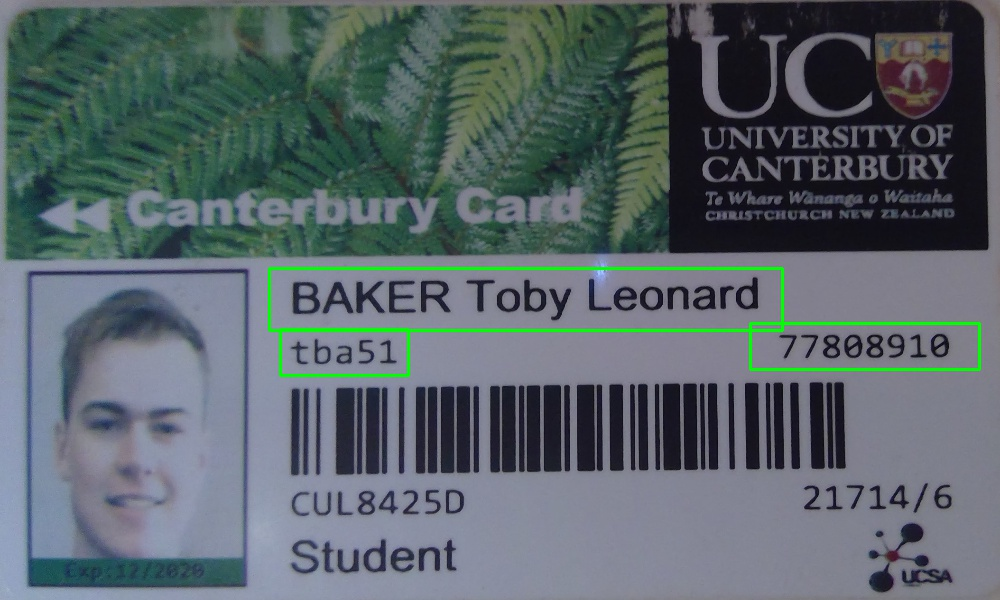
\includegraphics[width=\linewidth]{ID-Bounding-Box.jpg}
  		\caption{UC ID card showing regions of interest}
  		\label{fig:BoundingID}
	\end{figure}	

	\section{Background}

Liu and Samarabandu [6] proposed a multi-scale edge-based text extraction algorithm, which can efficiently localize text in both documents as well as indoor/outdoor scenes. It is designed to be robust in any scenario and can account for variations in orientation, font, size and alignment. They begin by using the edge strength, density and orientation variance to find candidate text regions. Following this they localize these regions and then perform character recognition. By performing a convolution operation with the compass operator seen in Figure 2, the characteristic properties of text are amplified. 

	\subsection{Pre-Processing}

Firstly, a Gaussian blur using a five by five kernel is applied to the captured image to reduce noise and detailed regions. Gaussian blur reduces the effect of a pixel the further the pixel is from the centre of the kernel [11]. 
Following the blurring process, the image is converted to greyscale and thresholded. Thresholding is used as we are only interested in areas of white and black. After image blurring the pixels surrounding areas of thin text are slightly greyed. When thresholding is carried out these pixels will become black, thickening thin areas or text to assist the optical character recognition.

	\subsection{Text Region Localization}



	
\end{document}
